%% LaTeX-Beamer template for KIT design
%% by Erik Burger, Christian Hammer
%% title picture by Klaus Krogmann
%%
%% version 2.0
%%
%% mostly compatible to KIT corporate design v2.0
%% http://intranet.kit.edu/gestaltungsrichtlinien.php
%%
%% Problems, bugs and comments to
%% burger@kit.edu

\documentclass[18pt]{beamer}
\usepackage{subfigure}					% Sub floats
\usepackage{listings}                   % Source Code
\lstset{ %
language=XML,               	 % the language of the code
%basicstyle=\footnotesize,       % the size of the fonts that are used for the code
basicstyle=\ttfamily\fontsize{6}{8}\selectfont,       % the size of the fonts that are used for the code
%numbers=left,                   % where to put the line-numbers
numbers=none,
numberstyle=\footnotesize,      % the size of the fonts that are used for the line-numbers
stepnumber=2,                   % the step between two line-numbers. If it's 1, each line 
                                % will be numbered
numbersep=5pt,                  % how far the line-numbers are from the code
backgroundcolor=\color{white},  % choose the background color. You must add \usepackage{color}
showspaces=false,               % show spaces adding particular underscores
showstringspaces=false,         % underline spaces within strings
showtabs=false,                 % show tabs within strings adding particular underscores
frame=single,                   % adds a frame around the code
tabsize=2,                      % sets default tabsize to 2 spaces
captionpos=b,                   % sets the caption-position to bottom
breaklines=true,                % sets automatic line breaking
breakatwhitespace=false,        % sets if automatic breaks should only happen at whitespace
%~ title=\lstname,                 % show the filename of files included with \lstinputlisting;
                                % also try caption instead of title
title=OWL Axioms,
escapeinside={\%*}{*)},         % if you want to add a comment within your code
morekeywords={*,...},           % if you want to add more keywords to the set
linewidth=6cm					% frame size
}
\usetheme{kit}
\usepackage{color}

%% TITLE PICTURE

% if a custom picture is to be used on the title page, copy it into the 'logos'
% directory, in the line below, replace 'mypicture' with the 
% filename (without extension) and uncomment the following line
% (picture proportions: 63 : 20, *.eps format if you use latex+dvips+ps2pdf,
% *.jpg/*.png/*.pdf if you use pdflatex)

%\titleimage{mypicture}

%% TITLE LOGO

% for a custom logo on the front page, copy your file into the 'logos'
% directory, insert the filename in the line below and uncomment it

\titlelogo{fzilogo}

% (*.eps format if you use latex+dvips+ps2pdf,
% *.jpg/*.png/*.pdf if you use pdflatex)

%% BIBTEX ICON/KEY

% if you want to see BibTeX keys in the references view instead of the symbol,
% uncomment the following line
% \usebibitemtemplate{\insertbiblabel}

% the presentation starts here

\title[Replica Framework]{Replica Framework}
\subtitle{A Framework for Ontology Sharing and Distributed Ontology Systems}
\author{Jan Novacek}

\institute{FZI Department for Information Process Engineering}

\begin{document}

% change the following line to "ngerman" for German style date and logos
\selectlanguage{english}

%title page
\begin{frame}
\titlepage
\end{frame}

%table of contents
\frame{
\frametitle{Outline}
\tableofcontents
}

\section{Introduction}
\subsection{Semantic Web}
\frame{
	\frametitle{Semantic Web}
%	\begin{block}{Semantic Web}
		\begin{itemize}
			\item Plenty of information on the internet today,
				information representations are designed to be used by humans.
				\begin{figure}
					\begin{center}
						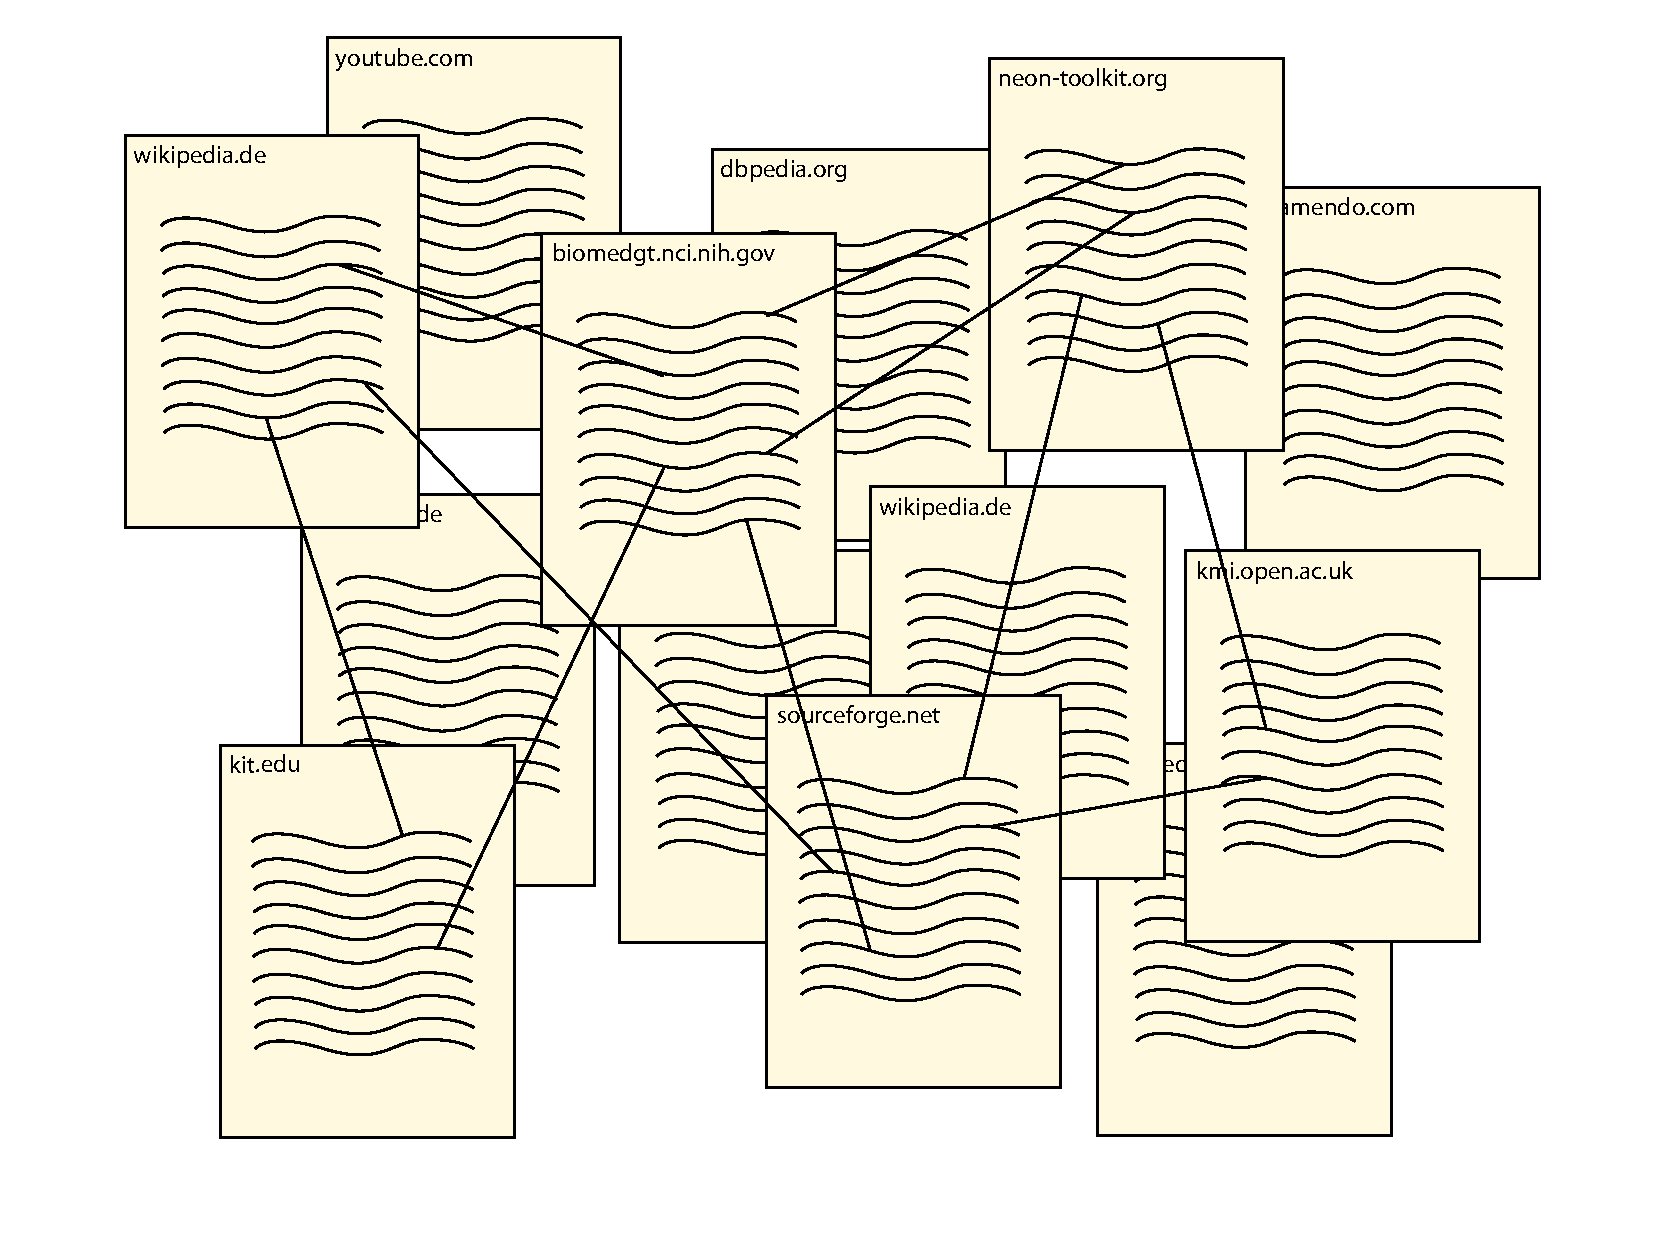
\includegraphics[width=5cm]{BilderSemanticWeb/SemanticWeb.pdf}
						\includegraphics[width=4cm]{BilderSemanticWeb/internet-map.jpg}
					\end{center}
				\end{figure}
%			\item Within the semantic web effort languages for expressing
%				such knowledge in a machine processable form are developed.
			\item The approach of the Semantic Web is to augment the
				existing web with machine processable meta information
				\cite{berners-lee98}.
		\end{itemize}
%	\end{block}
}
\subsection{Ontologies}
\frame{
	\frametitle{Ontologies}
		\begin{block}{Ontologies}
			\begin{itemize}
				%~ \item In computer science an ontology is a \emph{”formal, explicit
					%~ specification of a shared conceptualization”} \cite{gruber1993}.
				\item Used to represent knowledge in a machine readable form.
				\item Knowledge modeled as a set of concepts and the relations between these concepts.
				\item Reasoning systems can be used to infer additional knowledge.
			\end{itemize}
			%~ \begin{tabular}{|l|r|}
			%~ xxxxxxxx\=xxxxxxxx\kill
				%~ 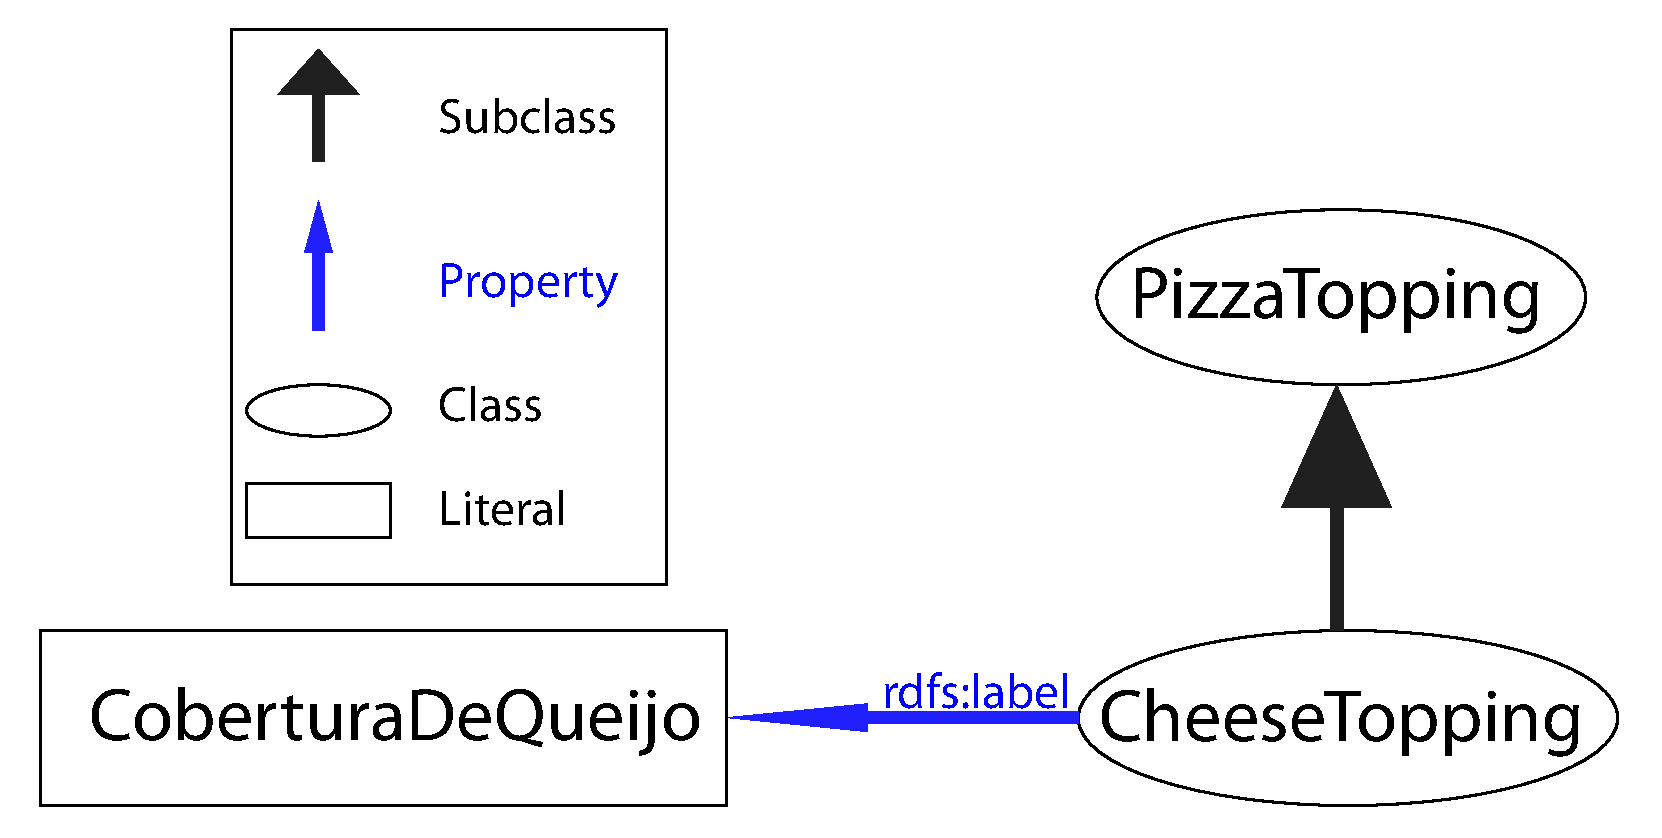
\includegraphics[width=4cm]{BilderSemanticWeb/Ontology-english.pdf}\>
				%~ \lstinputlisting{owlclass.lst}
			%~ \end{tabular}
		\end{block}
		\begin{block}{Example}
			\begin{tabular}{r r}
				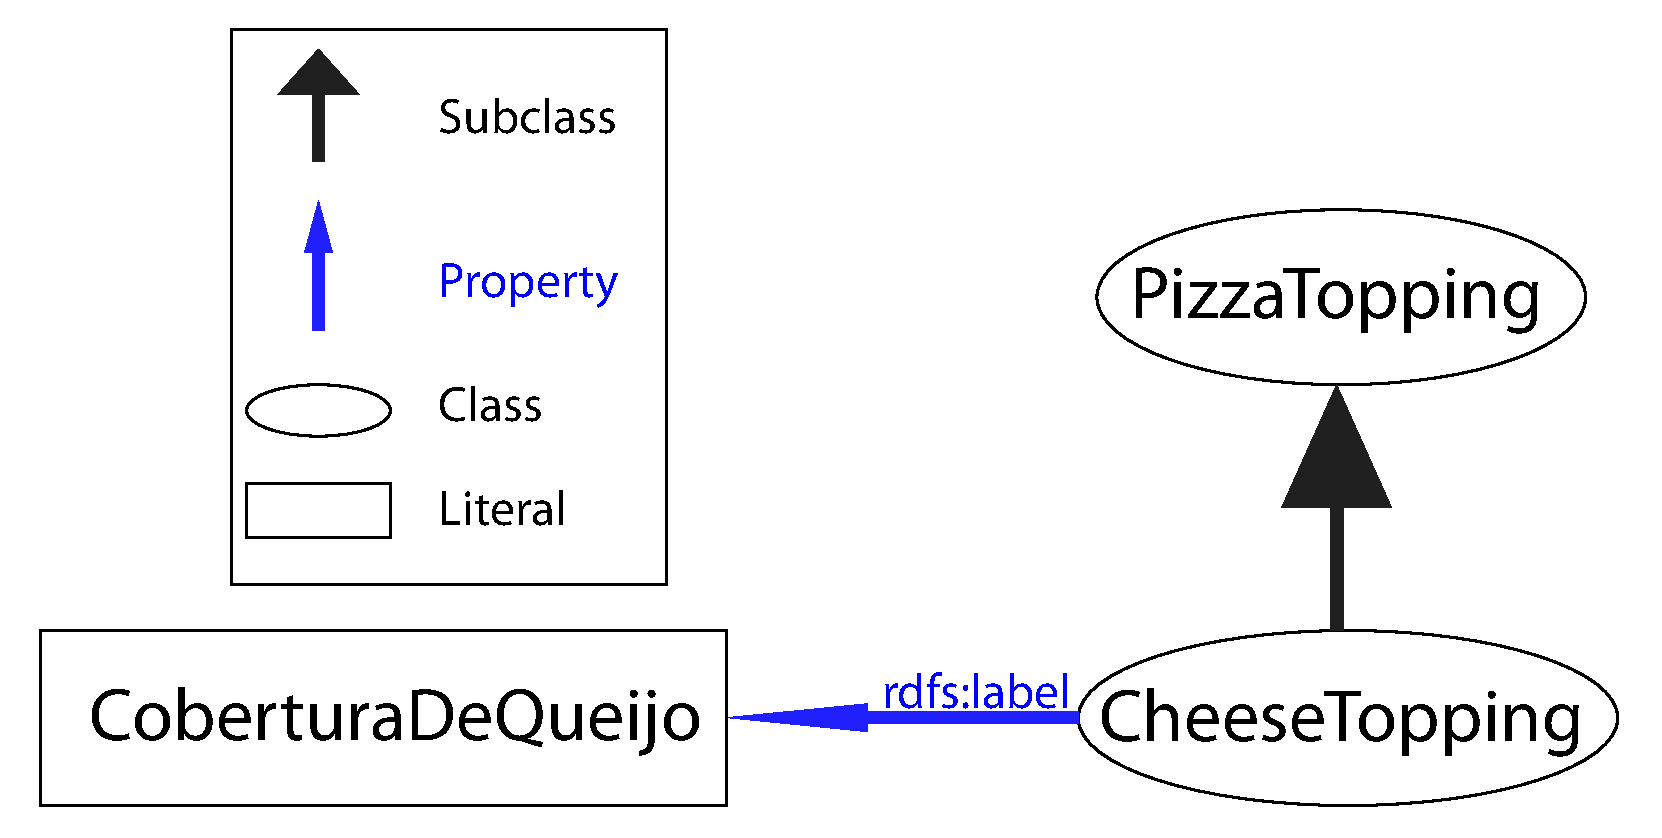
\includegraphics[width=4cm]{BilderSemanticWeb/Ontology-english.pdf} &
				\lstinputlisting{owlclass.lst}
			\end{tabular}
		\end{block}
		%~ \begin{figure}
			%~ \centering
			%~ \subfigure[Blub]{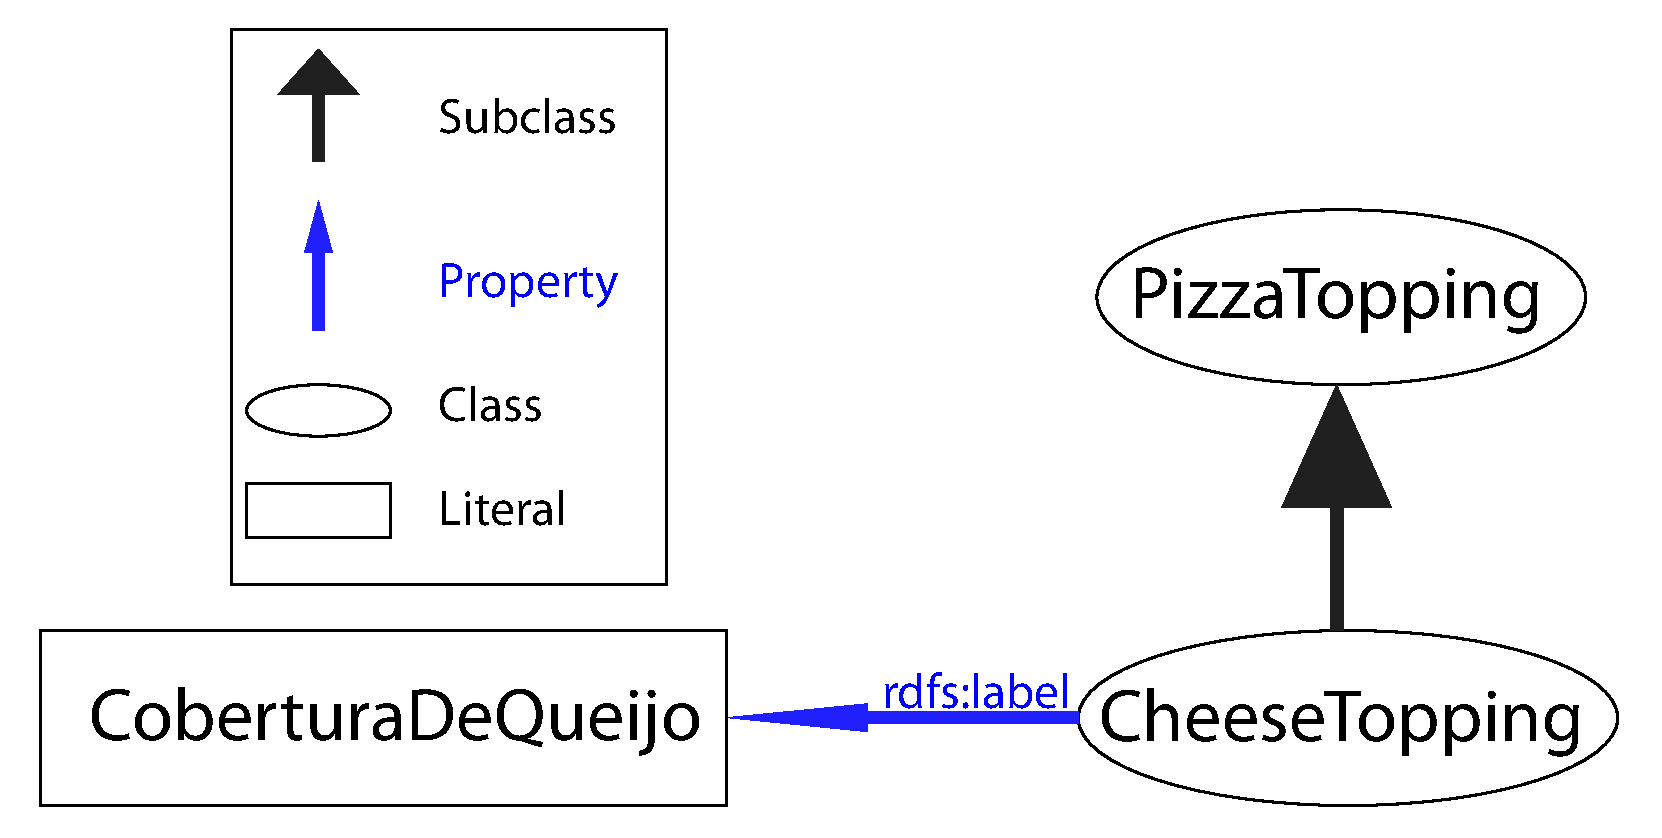
\includegraphics[width=4cm]{BilderSemanticWeb/Ontology-english.pdf}}
			%~ \subfigure[Blub2]{\lstinputlisting{owlclass.lst}}
		%~ \end{figure}
%~ \subsection{Semantic Web}
%~ \frame{
	%~ \frametitle{Semantic Web}
	%~ \begin{block}
		%~ \begin{itemize}
			%~ \item One problem with information on the internet today is that
				%~ information representations are	designed to be used by humans.
			%~ \item Within the semantic web effort languages for expressing
				%~ such knowledge in a machine processable form are developed.
		%~ \end{itemize}
	%~ \end{block}
%~ }
}
\section{Motivation}
\frame{
	\frametitle{Motivation 1/2}
	An example for a large, complex ontology is BiomedGT
	\includegraphics[width=1.5cm]{logos/biomedgt-logo.jpg}\\
	\begin{itemize}
	   \item New terminology aimed at supporting translational research
%~ research more quickly and efficiently into medical practice and, thus,
%~ meaningful health outcomes, whether those are physical, mental, or social outcomes
	   \item Collaborative Ontology Development Wiki
		\item Ontology experts incorporate and integrate changes
		\item Builds on the strengths of the NCI Thesaurus\footnote{\tiny The NCI
		   Thesaurus covers vocabulary for clinical care, translational and basic
		   research, and public information and administrative activities, see
		   \url{http://ncit.nci.nih.gov/ncitbrowser/}}
	\end{itemize}
%~	\rotatebox{0}{
%~			\resizebox{!}{0.6\textwidth}{
		\fbox{
				\includegraphics[width=3.5cm]{BilderSemanticWeb/BiomedGT-screenshot.png}
		}
%~			}
%~	}
%~	\rotatebox{0}{
%~			\resizebox{!}{0.6\textwidth}{
		\fbox{
				\includegraphics[width=4cm]{BilderSemanticWeb/Protege-screenshot.png}
		}
%~			}
%~	}
}
%~\subsection{blub}
\frame{
	\frametitle{Motivation 2/2}
	\begin{block}{Collaborative Ontology Development (COD)}
		\begin{itemize}
			\item \uppercase{\textbf{why}} Ontology development very
				hard or impossible for a single person.
			%~ \pause
			\item \uppercase{\textbf{what}} In collaborative work, communication is essential.
			%~ \pause
			\item \uppercase{\textbf{how}} Supplying chats, message boards and other tools
				which assist communication and matters to work collaboratively.
			%~ \pause
		\end{itemize}
	\end{block}
	\begin{block}{Distributed Ontology System (DOS)}
		\begin{itemize}
			\item \uppercase{\textbf{why}} Handle very large Ontologies.
			%~ \pause
			\item \uppercase{\textbf{why}} Performance of current reasoners is not sufficient \cite{chen09}.
			%~ \pause
			\item \uppercase{\textbf{how}} Scatter data and
				query processing across a set of nodes.
		\end{itemize}
	\end{block}
}
\subsection{Purpose and Contribution}
\frame{
	\frametitle{Purpose and Contribution}
	\begin{block}{Purpose}
		\begin{itemize}
			\item A novel framework for developing a Distributed Ontology System
				(DOS) and tools for Collaborative Ontology Development (COD).
			%~ \pause
			\item An initial step to met requirements of both fields.
		\end{itemize}
	\end{block}
	\begin{block}{Contribution}
		\begin{itemize}
			\item Providing a toolset for developers.
			\item Supporting the Semantic Web effort.
		\end{itemize}
	\end{block}
}
\subsection{Usage scenarios}
\frame{
	\frametitle{Usage scenarios}
	\rotatebox{0}{
			\resizebox{!}{0.6\textwidth}{
					\fbox{
							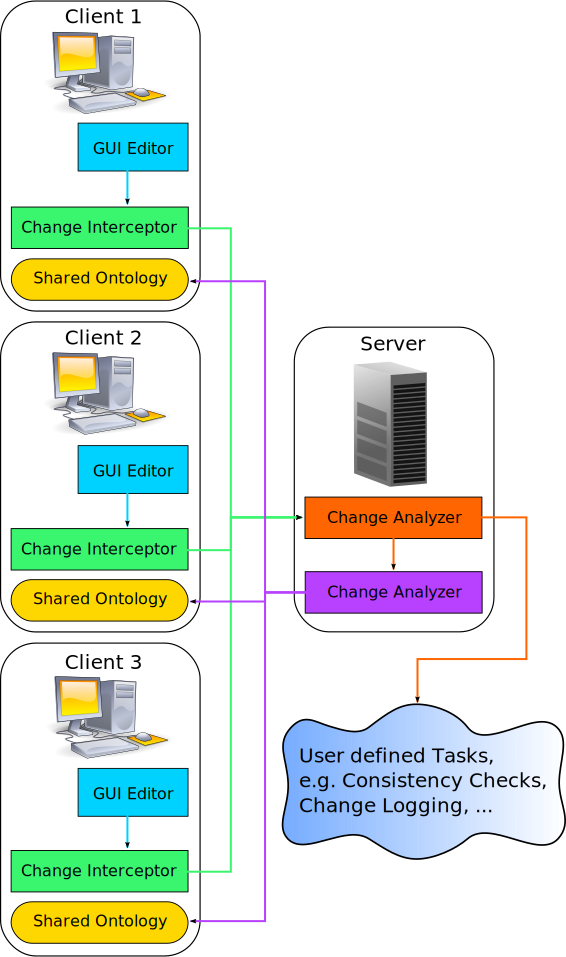
\includegraphics{BilderFrameworkArch/scenario0.pdf}
					}
			}
	}
	\rotatebox{0}{
			\resizebox{!}{0.6\textwidth}{
					\fbox{
							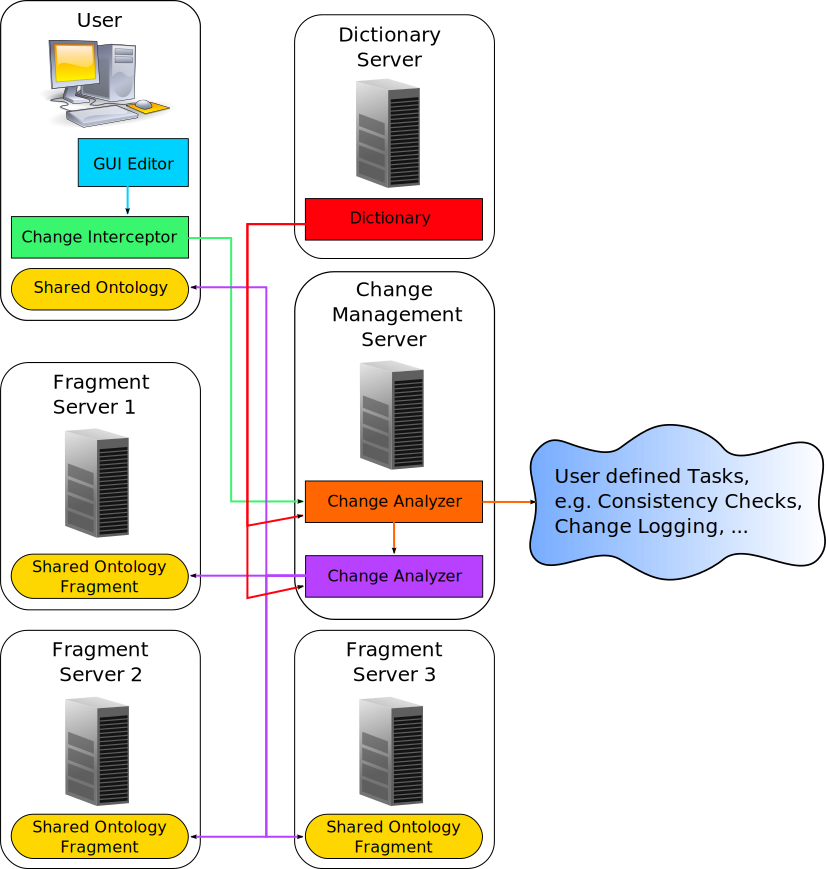
\includegraphics{BilderFrameworkArch/scenario1.pdf}
					}
			}
	}
}
%~ \subsection{Components}
%~ \frame{
	%~ \frametitle{Framework components}
	%~ The core components of the framework are:
	%~ \begin{block}{Distributed Ontology System}
		%~ \begin{itemize}
			%~ \item Shared Ontology, Shared Ontology Fragment
			%~ \pause
			%~ \item Dictionary
			%~ \pause
			%~ \item Change Interceptor
			%~ \pause
			%~ \item Change Analyzer
			%~ \pause
			%~ \item Change Propagator
			%~ \pause
			%~ \item Communication Node - Server and Client
		%~ \end{itemize}
	%~ \end{block}
%~ }

\section{Demonstrators}
\subsection{Standalone}
\frame{
	\frametitle{Standalone Demonstrator}
	The Replica Framework demonstrator is a standalone application meant
	to demonstrate and test the Replica Framework implementation.
	\begin{figure}[h]
        \begin{center}
                \includegraphics[width=8cm]{BilderFrontendImpl/demonstrator.png}
        \end{center}
        %~ \label{fig_demo}
	\end{figure}
	%~ \includegraphics[width=14mm]{logos/kitlogo_en_rgb} 
}
\subsection{NeOn Toolkit Plugin}
\frame{
	\frametitle{NeOn Toolkit Plugin}
	For demonstration purposes and evaluating the framework in a real-world
	application, a plug-in for the NeOn Toolkit\footnote{Ontology engeneering
	environment developed as part of the NeOn Project,
	\url{http://neon-toolkit.org/}} Platform has been implemented.
	\begin{figure}
		\begin{center}
				\includegraphics[width=4cm]{BilderFrontendImpl/wizard0.png}
				\vspace{1cm}
				\includegraphics[width=4cm]{BilderFrontendImpl/wizard1.png}
		\end{center}
	\end{figure}
	%~ \end{block}
	%~ \begin{figure}[h]
        %~ \caption{Shared ontology creation wizard}
        %~ \centering
                        %~ \subfloat[Shared ontology project creation wizard.]{\includegraphics[width=0.45\textwidth]{BilderFrontendImpl/wizard0.png}}
                        %~ \hspace{1cm}
                        %~ \subfloat[Shared ontology project creation wizard.]{\includegraphics[width=0.45\textwidth]{BilderFrontendImpl/wizard1.png}}
        %~ \label{fig_sharedontowizard}
	%~ \end{figure}
}
\frame{
	%~ \frametitle{NeOn Toolkit Plugin}
	%~ For demonstration purposes and evaluating the framework in a real-world
	%~ application, a plug-in for the NeOn Toolkit Platform has been implemented.
	\begin{figure}[h]
		\begin{center}
				\includegraphics[width=0.8\textwidth]{BilderFrontendImpl/editor.png}
		\end{center}
	\end{figure}
}

\section{Conclusions}
%~ \subsection{Conclusions}
\frame{
	\frametitle{Conclusions}
	\begin{block}{Status}
		\begin{itemize}
			\item Framework concept and implementation, demonstrators.
			%~ \pause
			%~ \item \emph{Query management}, \emph{policy management} and
			   %~ private/shared workspace support have not been addressed
			\item Some aspects have not been addressed
				(\emph{Query management}, \emph{policy management} and
				private/shared workspace support).
			   %~ private/shared workspace
			%~ \pause
			\item Good performance in unit tests and demonstrators.\\
				Various improvement possibilities left.
		\end{itemize}
	\end{block}
	\begin{block}{Conclusions}
		\begin{itemize}
			\item Unified COD and DOS framework.
			%~ \pause
			\item High expandability.
			%~ \pause
			\item ECF-based implementation reliable basis for communication.
			%~ \pause
			\item Many features remain to be implemented in future work.
		\end{itemize}
	\end{block}
}

%~ \section{Section 1}
%~ \subsection{Subsection 1.1}
%~ \frame{
%~ \frametitle{Example slide A}
%~ \begin{itemize}
%~ \item PCM, Citation: \cite{becker2008a} %\language
%~ \pause
%~ \item Bullet point 2
%~ \item \dots
%~ \end{itemize}
%~ }
%~ \subsection{Subsection 1.2}
%~ \frame{
%~ \frametitle{Example slide B}
%~ \begin{block}{Block 1}
%~ \begin{itemize}
%~ \item Bullet point 1
%~ \pause
%~ \item Bullet point 2
%~ \item \dots
%~ \end{itemize}
%~ \end{block}
%~ }
%~ \section{Section 2}
%~ \frame{
%~ \frametitle{Example slide C}
%~ \begin{exampleblock}{Example 1}
%~ \begin{itemize}
%~ \item Bullet point 1
%~ \pause
%~ \item Bullet point 2
%~ \item \dots
%~ \end{itemize}
%~ \end{exampleblock}
%~ }
%~ \frame{
%~ \frametitle{Example slide D}
%~ \begin{alertblock}{Alert 1}
%~ \begin{itemize}
%~ \item Bullet point 1
%~ \pause
%~ \item Bullet point 2
%~ \item \dots
%~ \end{itemize}
%~ \end{alertblock}
%~ }

\section{Implementation Details}
\subsection{Technologies}
\frame{
	\frametitle{Technologies}
		The framework has been implemented in Java.\\
		%~ Main reason for chosing
		%~ Java was that the OWLAPI\footnote{Java API and reference implmentation for creating, manipulating and serialising OWL
%~ Ontologies, see \url{http://owlapi.sourceforge.net/}} is also implemented in Java.\\
		\vspace{0.2cm}
		Core technologies used:
	%~ \begin{block}{Collaborative Ontology Development (COD)}
		\begin{itemize}
			\item AspectJ, aspect-oriented programming,
				\includegraphics[width=1cm]{logos/aspectj-logo.png}\\
				$\rightarrow$ for implementing crosscutting-concerns.
			%~ \pause
			\item The Eclipse Communication Framework,
				\includegraphics[width=1cm]{logos/eclipse-logo.jpg}\\
				$\rightarrow$ providing a reliable basis for communication.
			%~ \pause
			\item Script languages integration Ruby and Groovy,
			\includegraphics[width=1.5cm]{logos/groovy-logo.png}
			\includegraphics[width=1.5cm]{logos/ruby-logo.jpg}\\
				$\rightarrow$ for rapid prototyping.
			%~ \pause
			\item OSGi service platform,\includegraphics[width=1.8cm]{logos/osgi-logo.png}\\
				$\rightarrow$ modular architecture and service platform.
		\end{itemize}
	%~ \end{block}
}
\subsection{Shared Ontology Implementation}
\frame{
	\frametitle{Shared Ontology Implementation}
	The shared ontology object is a fundamental component of the framework.
	To combine the OWLAPI \emph{OWLOntology} interface with the ECF \emph{ISharedObject} interface,
	the facade \emph{OWLReplicaOntology} was introduced.
	\begin{figure}[h]
		\begin{center}
				%~ \includegraphics[width=0.5\textwidth]{BilderBackendImpl/OWLReplicaOntology.png}
				\rotatebox{-90}{
					\resizebox{!}{0.6\textwidth}{
						\includegraphics{BilderBackendImpl/OWLReplicaOntology.pdf}
					}
				}
		\end{center}
	\end{figure}
	For implementing \emph{OWLReplicaOntology} the ECF class \emph{TransactionSharedObject}
	was extended, a reference implementation of the ECF \emph{ISharedObject} interface,
	in combination with the proxy pattern for delegating \emph{OWLOntology}
	method calls.
}
\subsection{Requirements met}
\frame{
	\frametitle{Requirements met}
	\begin{block}{General \cite{tudorache2010CollabProtege}}
		\begin{itemize}
			\item \textcolor{green}{Scalability, reliability and robustness}
			   \tiny by implementing Unit tests \normalsize
			\item \textcolor{green}{Support for various levels of expressiveness}
			   \tiny no restrictions in ontology development \normalsize
		\end{itemize}
	\end{block}
	\begin{block}{COD specific requirements \cite{tudorache2010CollabProtege}}
		\begin{itemize}
			\item \textcolor{red}{Access Control} \tiny granting access
            based on user IDs, fine grained control
			   by cross-cutting this concern with AspectJ \normalsize
			\item \textcolor{green}{Provenance of information} \tiny
			   by augmenting change data with meta information \normalsize
			\item \textcolor{green}{Communication tooling} \tiny by leveraging ECF
			   framework components \normalsize
		\end{itemize}
	\end{block}
	\begin{block}{DOS specific requirements \cite{hobo2004}}
		\begin{itemize}
			\item \textcolor{green}{Heterogeneity} \tiny by platform abstraction
			   and relying on asynchronous messaging \normalsize
			\item \textcolor{green}{Openness} \tiny by using open standarts and
			   simple APIs for all modules \normalsize
			\item \textcolor{green}{Transparency} \tiny by change filtering,
			   analyzing, logging \normalsize
			\item \textcolor{yellow}{Fault-Tolerance} \tiny
			   initial step: transactional messaging \normalsize
		\end{itemize}
	\end{block}
}

\section{References}
\frame{
\frametitle{References}
\bibliography{bibliography}
\bibliographystyle{ka-style}
%~ \bibliographystyle{plain} %does not render "url" fields...
%~ \bibliographystyle{IEEEtran}  %does render "url" fields, requires "_"s and "#"s to be escaped, e.g. "\_".
}

\frame{
	\centering
	\frametitle{License}
	\includegraphics[width=0.8cm]{logos/cc.pdf}
	\includegraphics[width=0.8cm]{logos/by.pdf}
	\includegraphics[width=0.8cm]{logos/sa.pdf}\\
	\tiny
	Dieses Werk von Jan Novacek steht unter einer Creative
	Commons Namensnennung-Weitergabe unter gleichen Bedingungen 3.0 Unported Lizenz.
	Um eine Kopie der Lizenz zu erhalten, gehen Sie bitte zu
	http://creativecommons.org/licenses/by-sa/3.0/de/ oder schreiben Sie an
	Creative Commons, 171
	Second Street, Suite 300, San Francisco, California 94105, USA.\\
	\vspace{1cm}
	\centering
	Davon ausgenommen sind die Logos von AspectJ, Ruby, Groovy, BiomedGT,\\
	das Bild der Internet Map auf Folie 3 sowie das KIT Beamer Theme.\\
	Hierf\"ur gelten die Lizenzen der jeweiligen Urheber.\\
}
\end{document}
